\presub
\subsection{Evaluation on Finding \taskone} \postsub
\label{eva_one}

\noindent\textbf{Parameter Setting:}
%We compare three frameworks: \sketchname, \EHname and \Splittername. For each frameworks, we using CM Sketch, CM-CU Sketch and Count Sketch approaches.
%
%We compare 5 approaches: CM \sketchname, CM-CU \sketchname, Count \sketchname, \EHname {} and \Splittername.
%
We compare 6 algorithms: \sketchname, \freCM\cite{cmsketch}, \freCU\cite{cusketch}, \freCF\cite{coldfilter}, \freSS\cite{spacesaving}, and \freunbia\cite{unbiasedsketch}.
For \freCM, \freCU{}, and \freCF, the parameters are set according to the recommendation of the authors.
In this experiment, we compare AAE, ARE, PR, CR, and insertion speed among the 6 algorithms.
The size of memory used ranges from 200KB to 400KB. We choose this range because: 1) \sketchname{} has performed well enough in this range and 2) relying on little memory will expose the difference between the algorithms.
			
\noindent\textbf{ARE (Figure~\ref{fre_are_syn}-\ref{fre_are_net}):}
We find that, on three real-world datasets, the ARE of \sketchname{} is around 3207 times, 708 times, 2735 times, 2707 times, and 2576 times lower than \freCM, \freCU, \freCF, \freSS{}, and \freunbia{}, respectively. On the synthetic dataset, the ARE of \sketchname{} is around 416 times, 74 times, 1851 times, 1866 times, and 1820 times lower than \freCM, \freCU, \freCF, \freSS{}, and \freunbia{}, respectively.
			
\noindent\textbf{PR (Figure~\ref{fre_pr_syn}-\ref{fre_pr_net}):}
We find that on three real-world datasets, the PR of \sketchname{} is around 11.2 times, 9.9 times, 2.8 times, 3.4 times, and 2.7 times higher than \freCM, \freCU, \freCF, \freSS{}, and \freunbia{} respectively. On the synthetic dataset, the PR of \sketchname{} is around 30.3 times, 33.8 times, 5.9 times, 5.5 times, and 5.8 times higher than \freCM, \freCU, \freCF, \freSS{}, and \freunbia{}, respectively.
	
\begin{figure*}[!ht]
	\centering
	%
	\subfigure[Synthetic dataset]{
		\begin{minipage}[t]{0.252\textwidth}{
		\prefig
		\begin{center}
		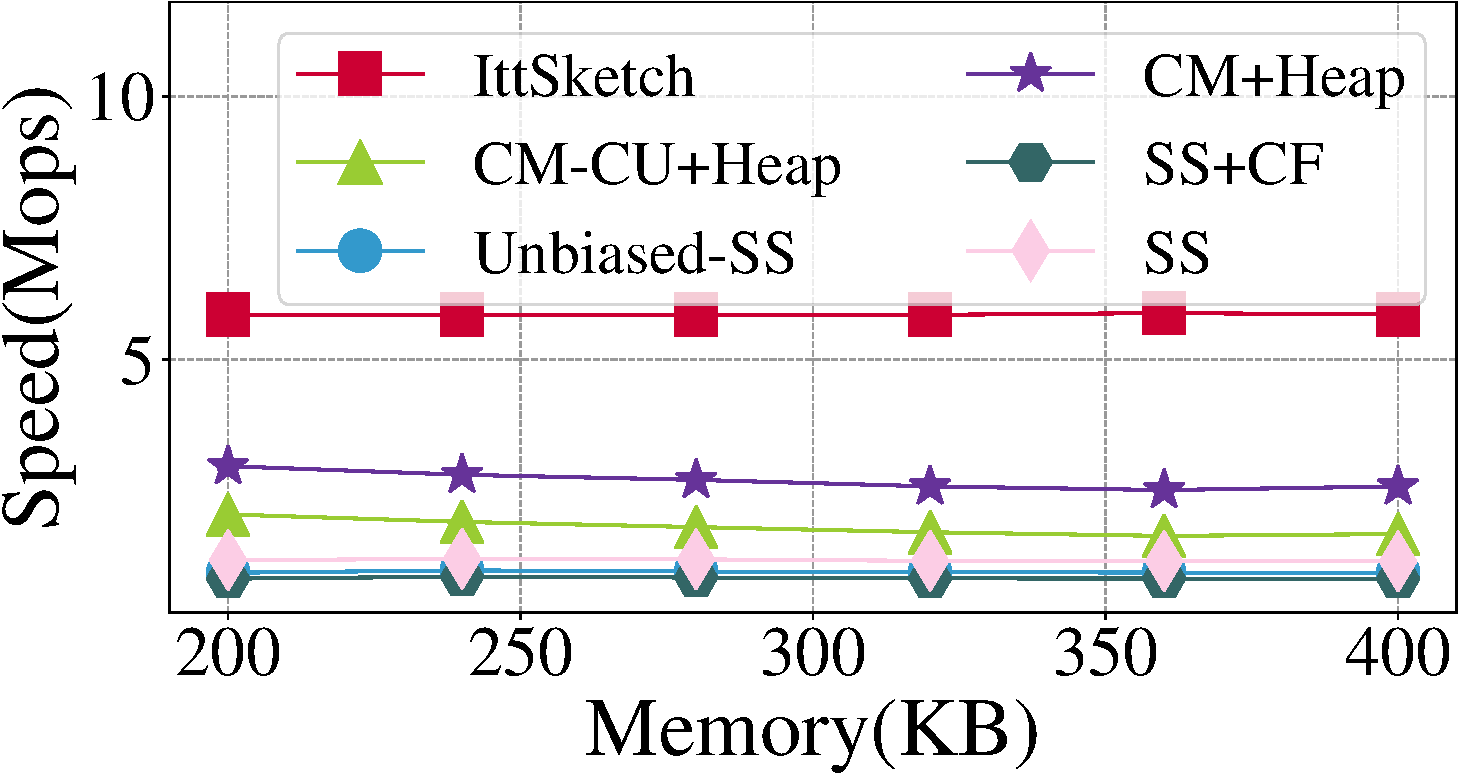
\includegraphics[width=0.95\textwidth, ]{Figures/fre/fre_speed/fre_syn_speed-cropped.pdf}
		\end{center}
		}
		\postfig 
		\adjustfigs
		\prefigcaption
		\label{fre_speed_syn}
		\postfigcaption
		\end{minipage}
	}
	%
	\subfigure[IP trace]{
		\begin{minipage}[t]{0.23\textwidth}{
		\prefig
		\begin{center}
		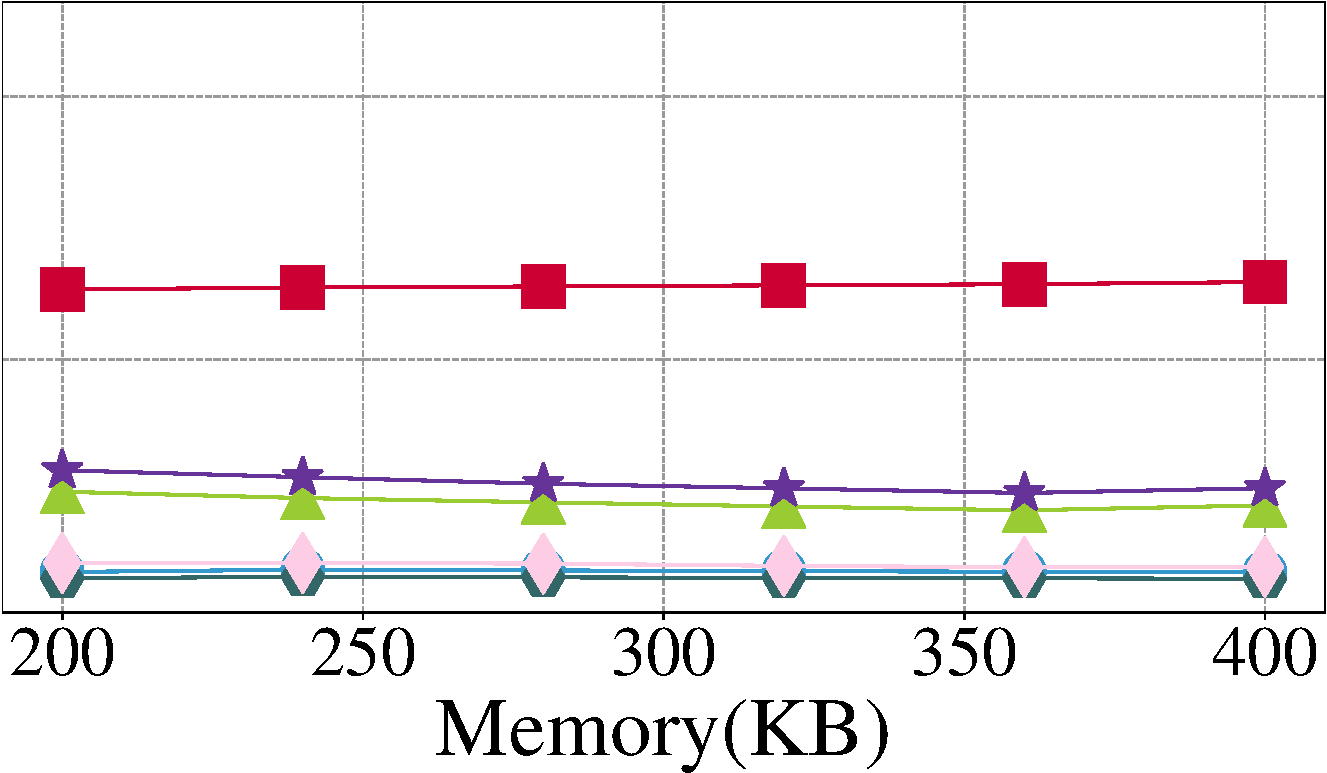
\includegraphics[width=0.95\textwidth, ]{Figures/fre/fre_speed/fre_ip_speed-cropped.pdf}
		\end{center}
		}
		\postfig
		\adjustfigs
		\prefigcaption
		\label{fre_speed_ip}\postfigcaption
		\end{minipage}
	}
	%
	\subfigure[Web page]{
		\begin{minipage}[t]{0.23\textwidth}{
		\prefig
		\begin{center}		
		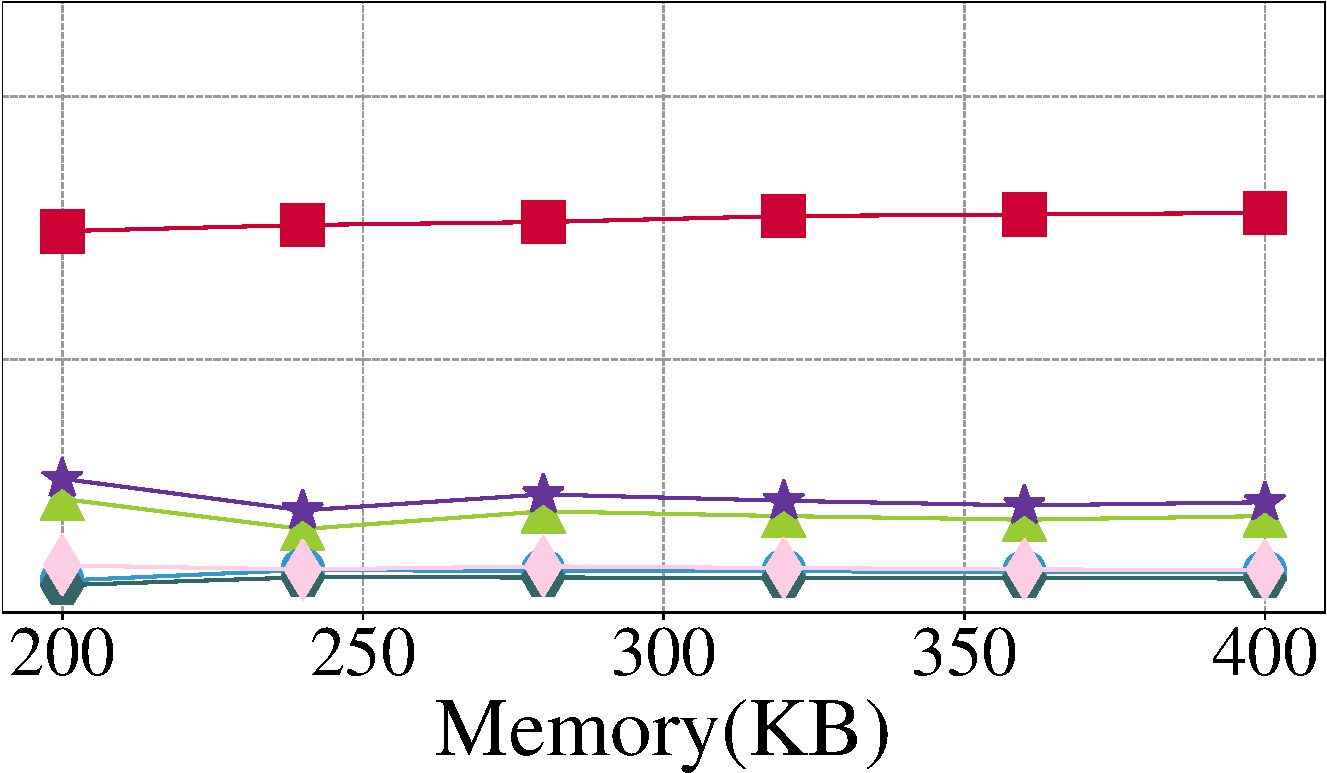
\includegraphics[width=0.95\textwidth, ]{Figures/fre/fre_speed/fre_web_speed-cropped.pdf}
		\end{center}
		}
		\postfig 
		\adjustfigs
		\prefigcaption
		\label{fre_speed_web}
		\postfigcaption
		\end{minipage}
	}
	%
	\subfigure[Network dataset]{
		\begin{minipage}[t]{0.23\textwidth}{
		\prefig
		\begin{center}		
		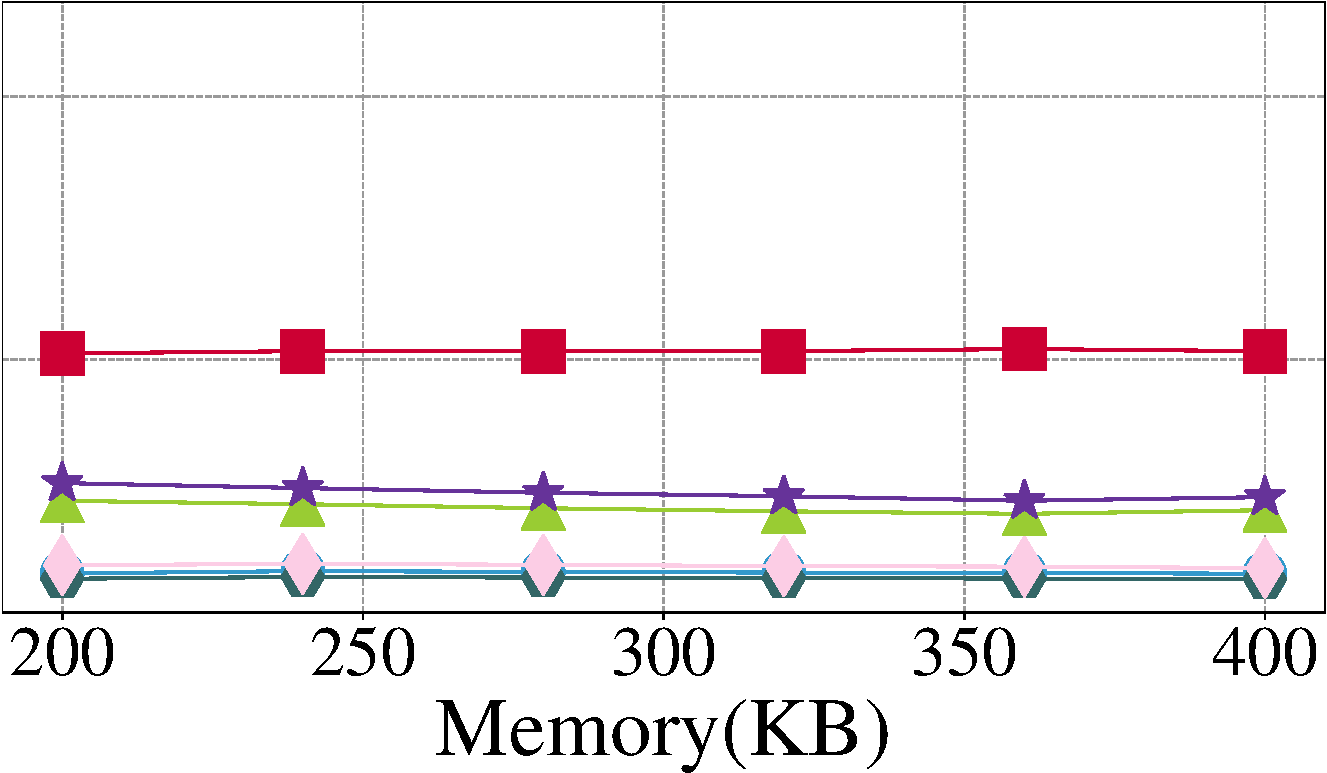
\includegraphics[width=0.95\textwidth, ]{Figures/fre/fre_speed/fre_net_speed-cropped.pdf}
		\end{center}
		}
		\postfig 
		\adjustfigs
		\prefigcaption
		\label{fre_speed_net}
		\postfigcaption
		\end{minipage}
	}
	\vvv \vvv
	\caption{Speed of finding \taskone.}
	\label{fre_speed}
\end{figure*}		
			
\noindent\textbf{Speed (Figure~\ref{fre_speed_syn}-\ref{fre_speed_net}):}
We find that, on three real-world datasets and one synthetic dataset, the insertion speed of \sketchname{} is around 2.2 times, 2.7 times, 7.7 times, 5.48 times, and 6.7 times faster than \freCM, \freCU, \freCF, \freSS{}, and \freunbia{}, respectively.


\noindent\textbf{AAE (Figure~\ref{fre_aae_syn}-\ref{fre_aae_net}) in Appendix \ref{app:fig}:}
We find that, on three real-world datasets, the AAE of \sketchname{} is around 7309 times, 995 times, 3860 times, 3701 times, and 3549 times lower than \freCM, \freCU, \freCF, \freSS{}, and \freunbia{}, respectively. Besides, on the synthetic dataset, the AAE of \sketchname{} is around 2278 times, 80 times, 3247 times, 3278 times, and 3205 times lower than \freCM, \freCU, \freCF, \freSS{}, and \freunbia{}, respectively. 

\begin{figure*}[!ht]
	\centering
	%
	\subfigure[Synthetic dataset]{
		\begin{minipage}[t]{0.255\textwidth}{
		\prefig
		\begin{center}
		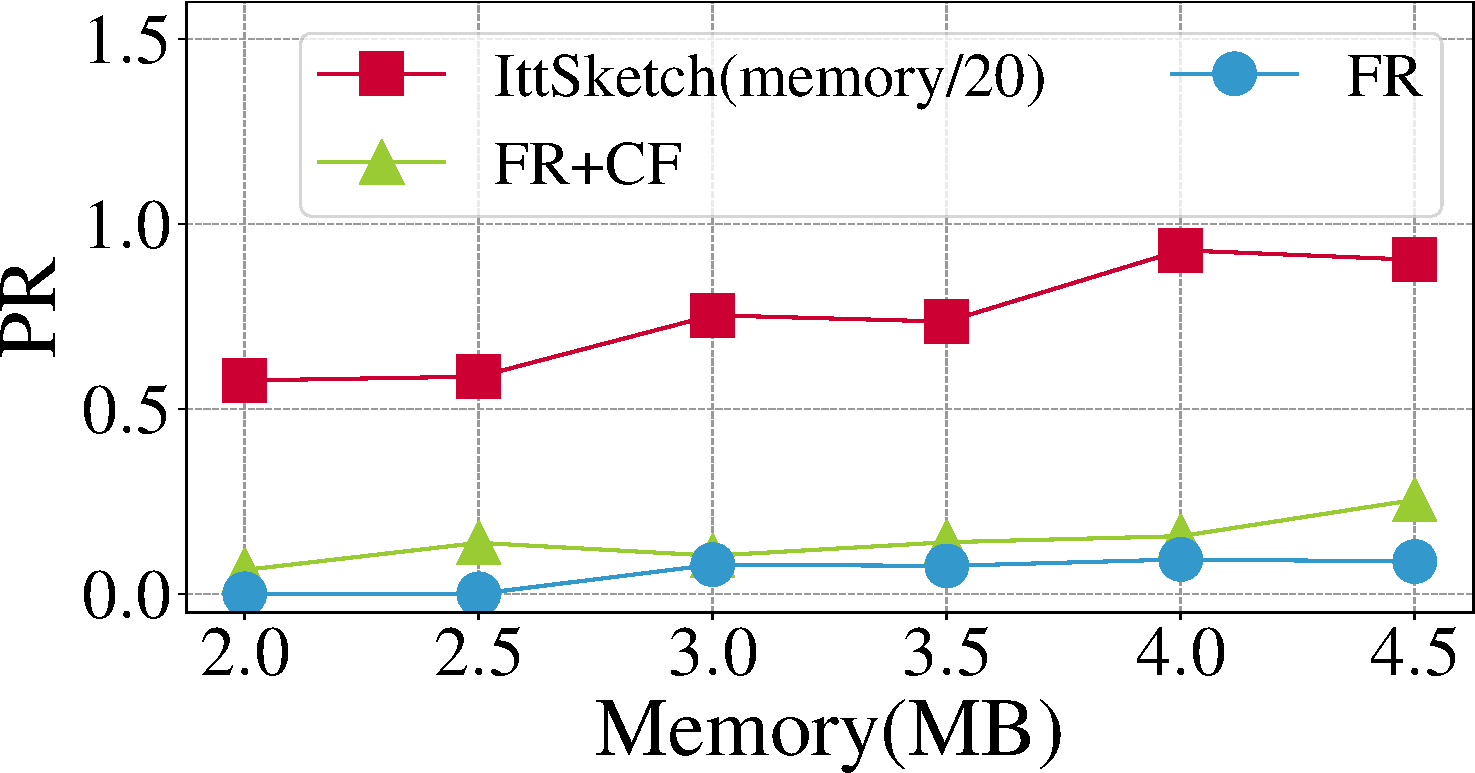
\includegraphics[width=0.95\textwidth, ]{Figures/cha/cha_pr/cha_syn_pr-cropped.pdf}
		\end{center}
		}
		\postfig 
		\adjustfigs
		\prefigcaption
		\label{cha_pr_syn}
		\postfigcaption
		\end{minipage}
	}
	%
	\subfigure[IP trace]{
		\begin{minipage}[t]{0.23\textwidth}{
		\prefig
		\begin{center}
		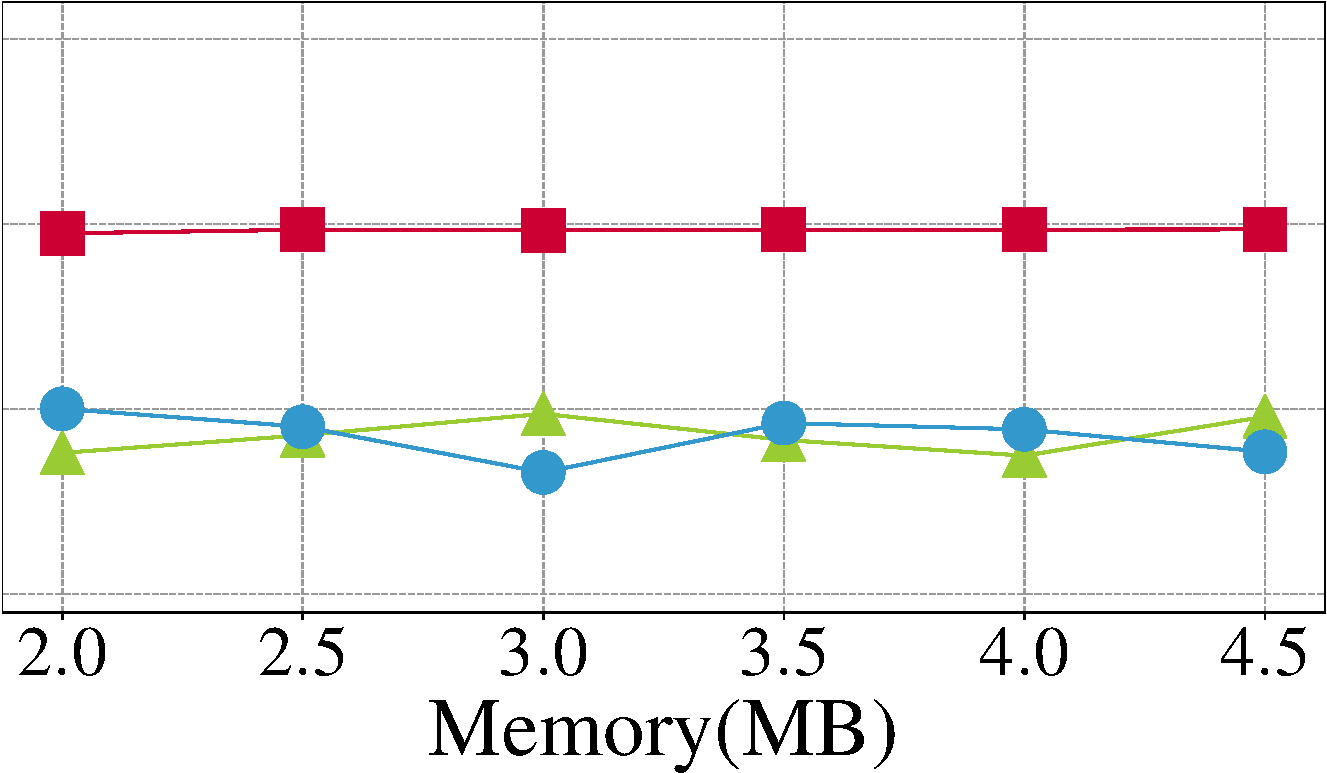
\includegraphics[width=0.95\textwidth, ]{Figures/cha/cha_pr/cha_ip_pr-cropped.pdf}
		\end{center}
		}
		\postfig
		\adjustfigs
		\prefigcaption
		\label{cha_pr_ip}
		\postfigcaption
		\end{minipage}
	}
	%
	\subfigure[Web page]{
		\begin{minipage}[t]{0.23\textwidth}{
		\prefig
		\begin{center}		
		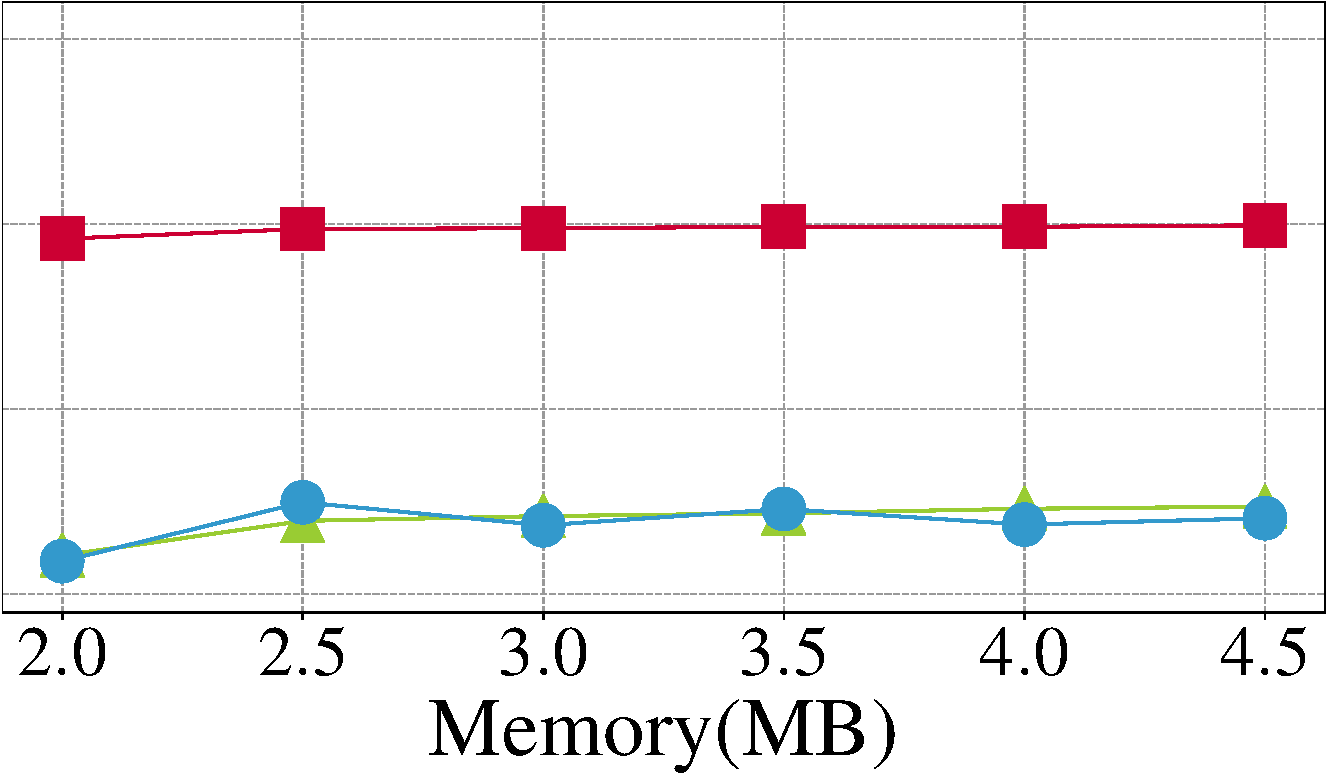
\includegraphics[width=0.95\textwidth, ]{Figures/cha/cha_pr/cha_web_pr-cropped.pdf}
		\end{center}
		}
		\postfig 
		\adjustfigs
		\prefigcaption
		\label{cha_pr_web}
		\postfigcaption
		\end{minipage}
	}
	%
	\subfigure[Network dataset]{
		\begin{minipage}[t]{0.23\textwidth}{
		\prefig
	    \begin{center}		
		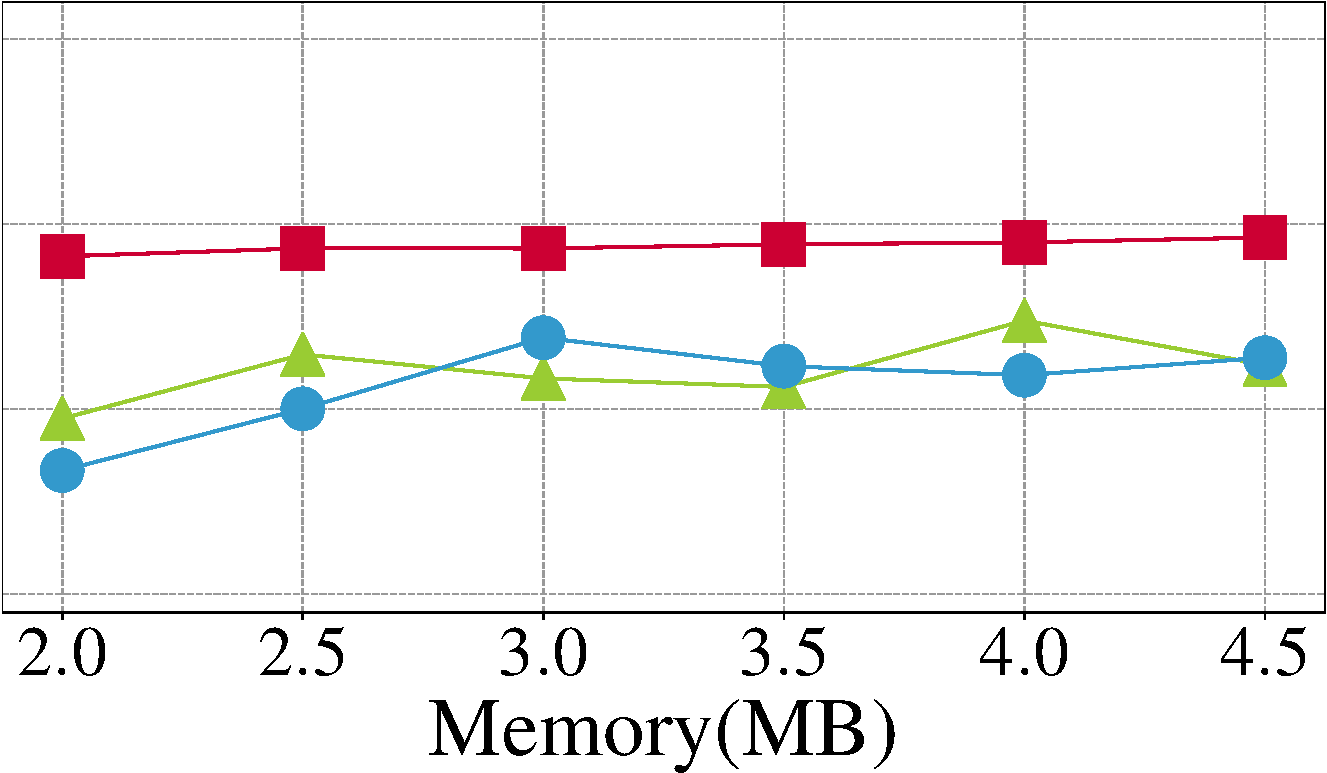
\includegraphics[width=0.95\textwidth, ]{Figures/cha/cha_pr/cha_net_pr-cropped.pdf}
		\end{center}
		}
		\postfig 
		\adjustfigs
		\prefigcaption
		\label{cha_pr_net}
		\postfigcaption
		\end{minipage}
	}
	%
	\vvv \vvv
    \caption{PR of finding \taskfour.}
	\label{cha_pr}
\end{figure*}

\begin{figure*}[!ht]
	\centering
	%
	\subfigure[Synthetic dataset]{
		\begin{minipage}[t]{0.24546\textwidth}{
		\prefig
		\begin{center}
		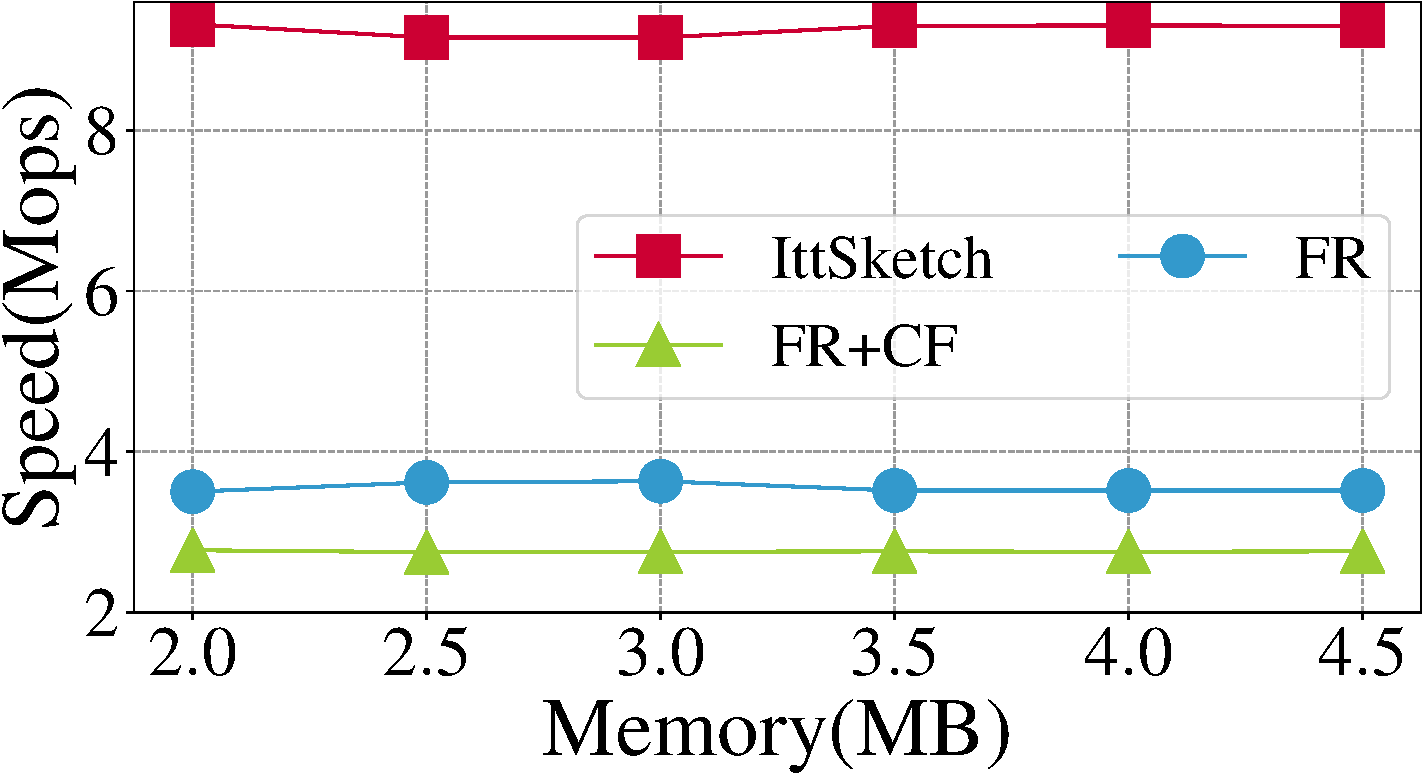
\includegraphics[width=0.95\textwidth, ]{Figures/cha/cha_speed/cha_syn_speed-cropped.pdf}
		\end{center}
		}
		\postfig 
		\adjustfigs
		\prefigcaption
		\label{cha_speed_syn}
		\postfigcaption
		\end{minipage}
	}
	%
	\subfigure[IP trace]{
		\begin{minipage}[t]{0.23\textwidth}{
		\prefig
		\begin{center}
		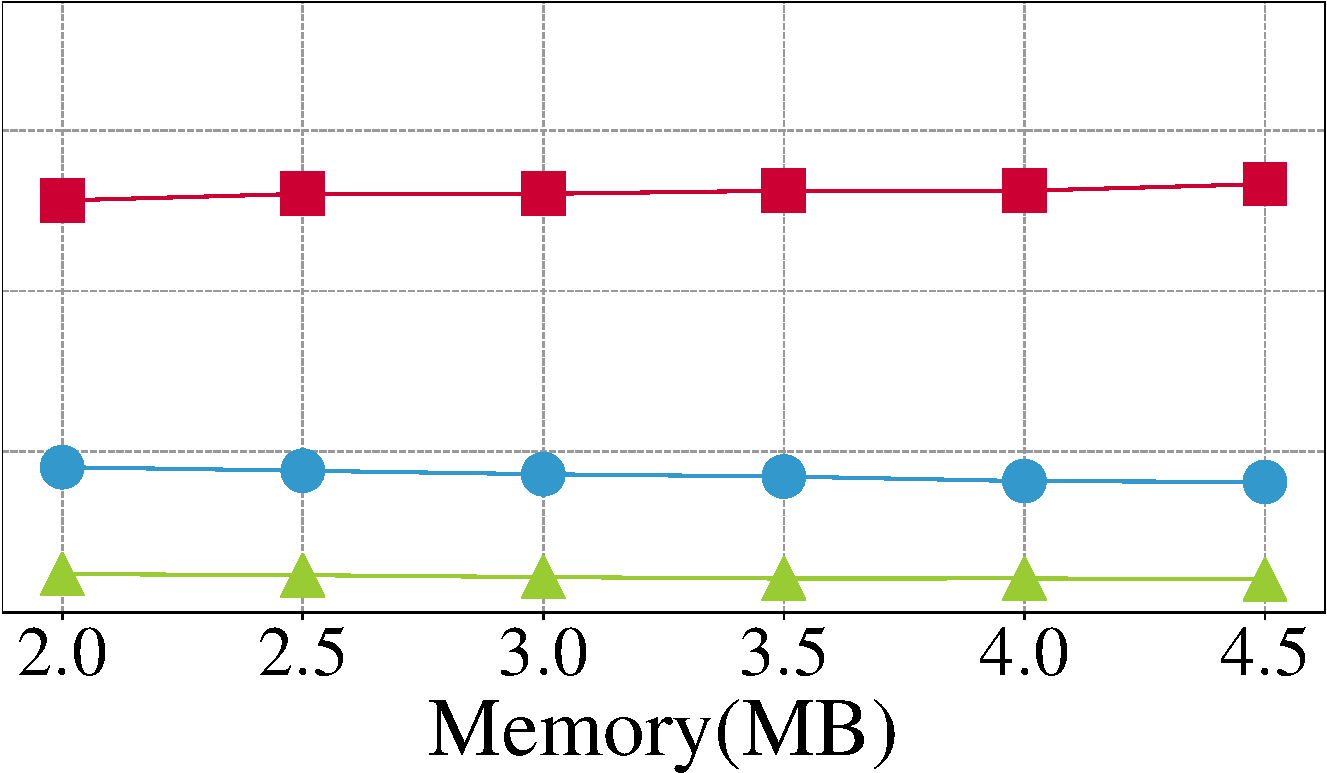
\includegraphics[width=0.95\textwidth, ]{Figures/cha/cha_speed/cha_ip_speed-cropped.pdf}
		\end{center}
		}
		\postfig
		\adjustfigs
		\prefigcaption
		\label{cha_speed_ip}
		\postfigcaption
		\end{minipage}
	}
	%
	\subfigure[Web page]{
		\begin{minipage}[t]{0.23\textwidth}{
		\prefig
		\begin{center}		
		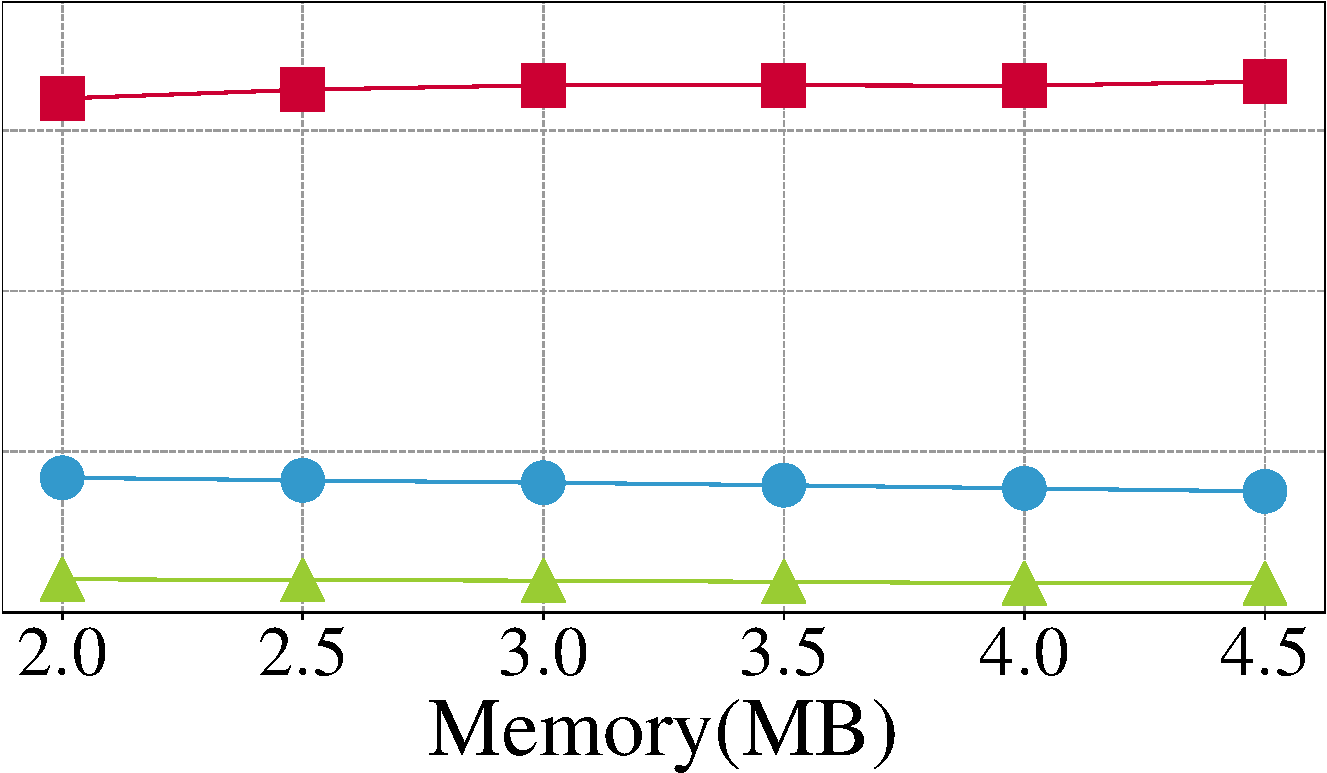
\includegraphics[width=0.95\textwidth, ]{Figures/cha/cha_speed/cha_web_speed-cropped.pdf}
		\end{center}
		}
		\postfig 
		\adjustfigs
		\prefigcaption
		\label{cha_speed_web}
		\postfigcaption
		\end{minipage}
	}
	%
	\subfigure[Network dataset]{
		\begin{minipage}[t]{0.23\textwidth}{
		\prefig
		\begin{center}		
		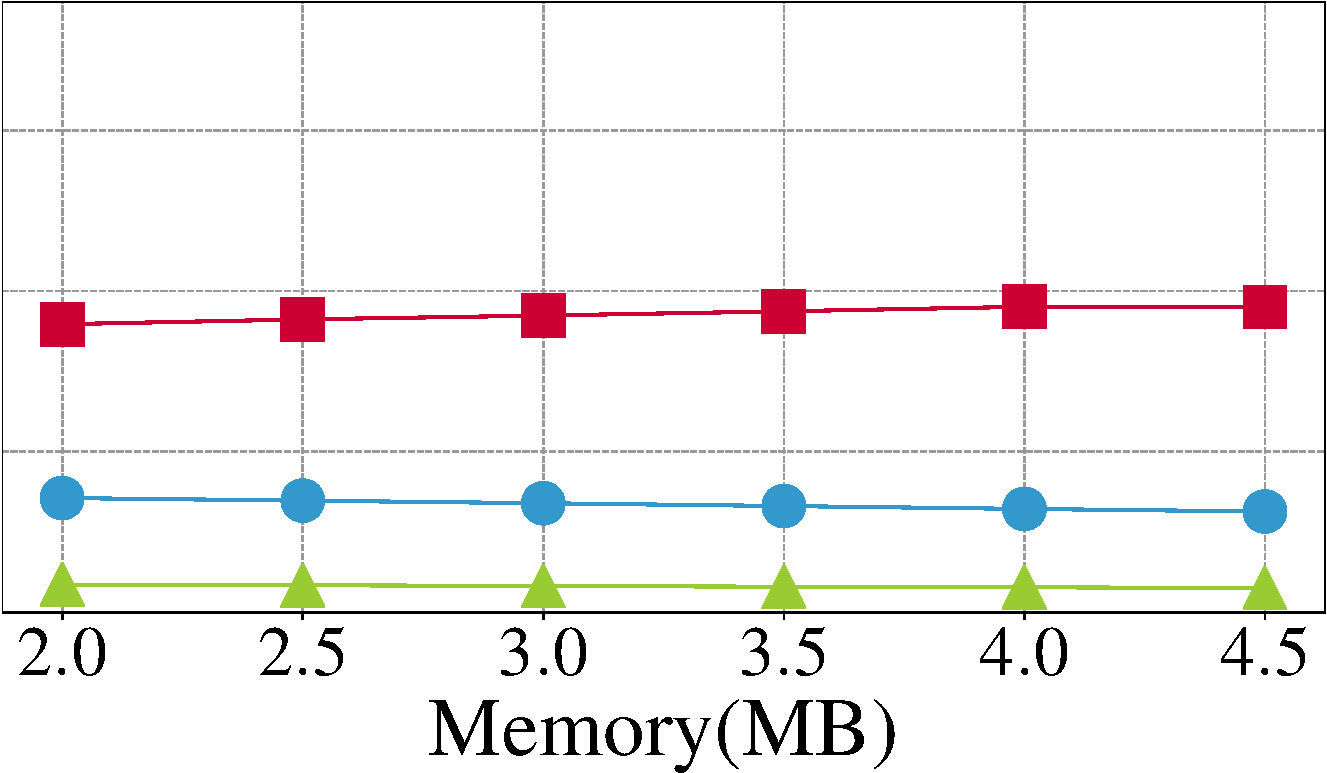
\includegraphics[width=0.95\textwidth, ]{Figures/cha/cha_speed/cha_net_speed-cropped.pdf}
		\end{center}
		}
		\postfig 
		\adjustfigs
		\prefigcaption
		\label{cha_speed_net}
		\postfigcaption
		\end{minipage}
	}
	%
	\vvv \vvv
    \caption{Speed of finding \taskfour.}
	\label{cha_speed}
\end{figure*}

\noindent\textbf{CR (Figure~\ref{fre_cr_syn}-\ref{fre_cr_net}) in Appendix \ref{app:fig}:}
We find that, on three real-world datasets, the CR of \sketchname{} is around 5.6 times, 5 times, 1.7 times, 2 times, and 1.6 times higher than \freCM, \freCU, \freCF, \freSS{}, and \freunbia{}, respectively. 
On the synthetic dataset, the CR of \sketchname{} is around 17 times, 18 times, 5 times, 4.7 times, and 5.3 times higher than \freCM, \freCU, \freCF, \freSS{}, and \freunbia{}, respectively.


\noindent\textbf{Summary:}
%
1) \sketchname{} can achieve high accuracy with limited memory. The ARE of \sketchname{} is lower than 0.01 when the memory is set to 200KB, while the ARE of the other algorithms is often higher than 1. As seen in the figures, the ARE of \freSS, \freCF{}, and \freunbia{} often exceed the range of the plots.

2) \sketchname{} can report more correct instances than other approaches. \sketchname{} often reports more than 99 percent of the correct instances, while the other approaches report less than 40 percent, because they often consume too much memory on the hash table or Stream-Summary.

3) \sketchname{} achieves higher precision in reported instances. The PR of \sketchname{} is often higher than 0.99, while the PR of other approaches is often less than 0.6 because they overestimate the results. 

4) The insertion speed of \sketchname{} is also faster than the other approaches for the same memory consumption on three real-world datasets and one synthetic dataset.